\subsection{Diagramas de Componentes y Conectores con Deployment}

\subsubsection{Nivel 0}

\begin{figure}[H]
  \centering
  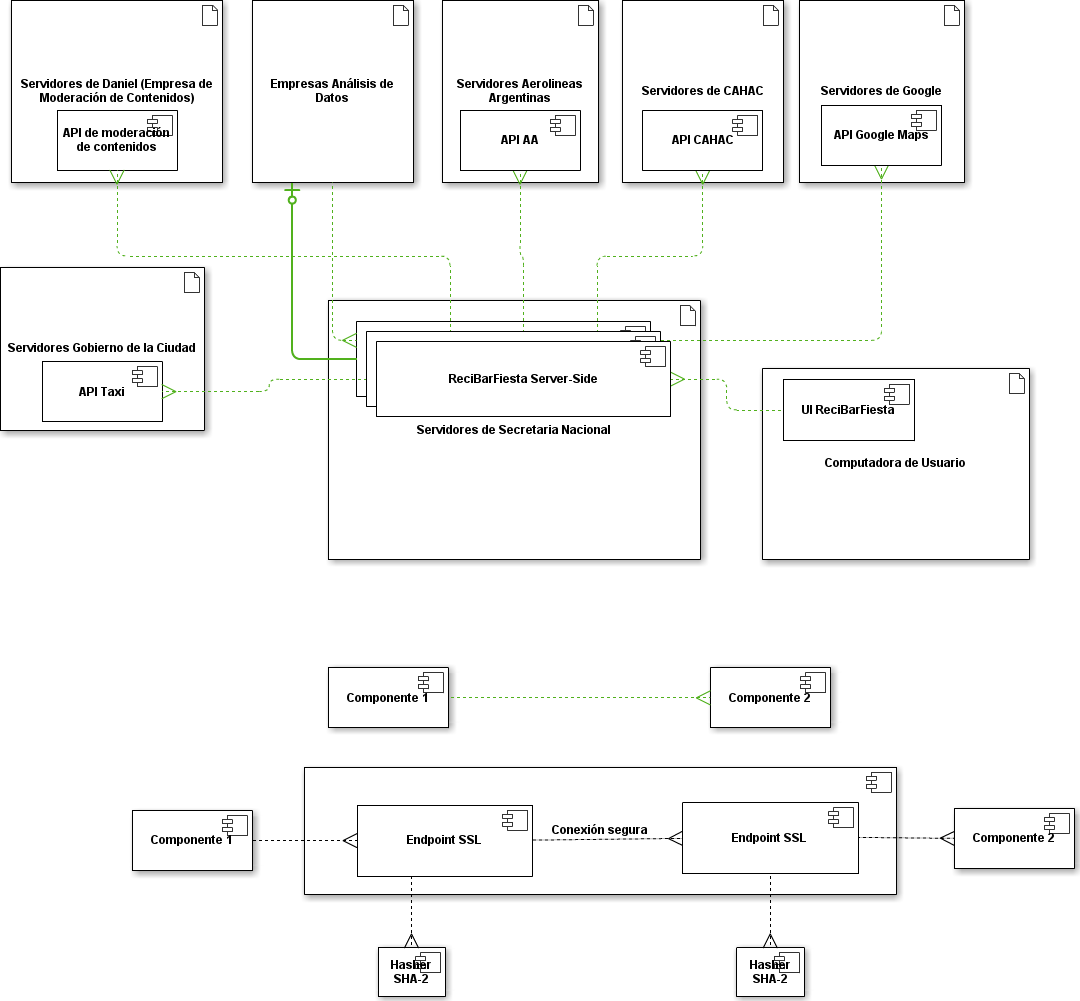
\includegraphics[width=\textwidth]{diagramas/Nivel0.png}
  \caption{\normalfont Vista de Nivel 0. Explicación del conector seguro.}
\end{figure} 


\subsubsection{ReciBarFiesta}

\begin{figure}[H]
  \centering
  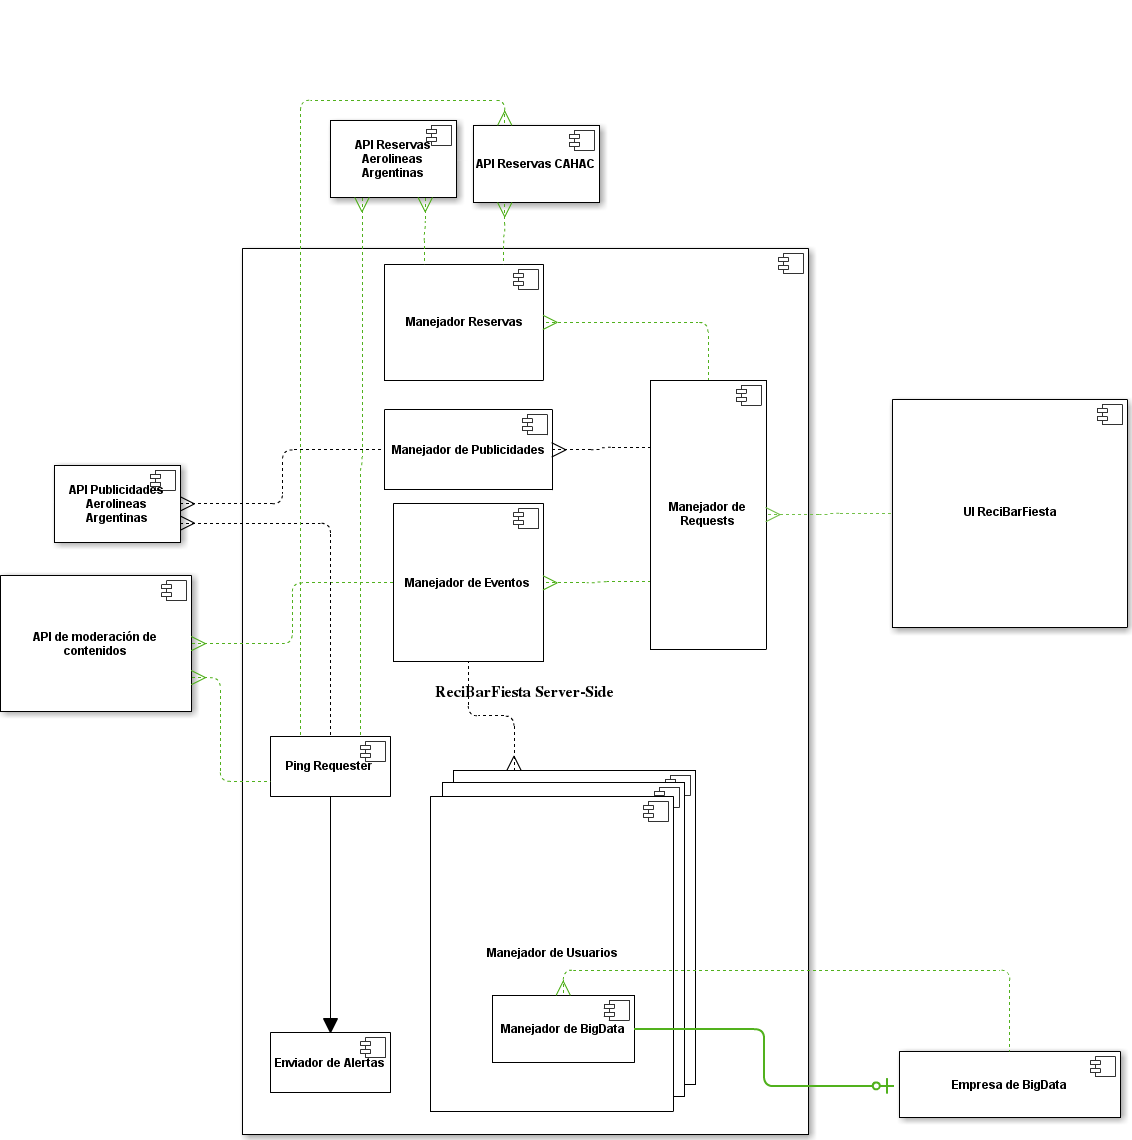
\includegraphics[width=\textwidth]{diagramas/ReciBarFiesta.png}
  \caption{\normalfont Vista de Nivel 1 de ReciBarFiesta del lado del servidor.}
\end{figure} 

\subsubsection{Manejador de Eventos}

\begin{figure}[H]
  \centering
  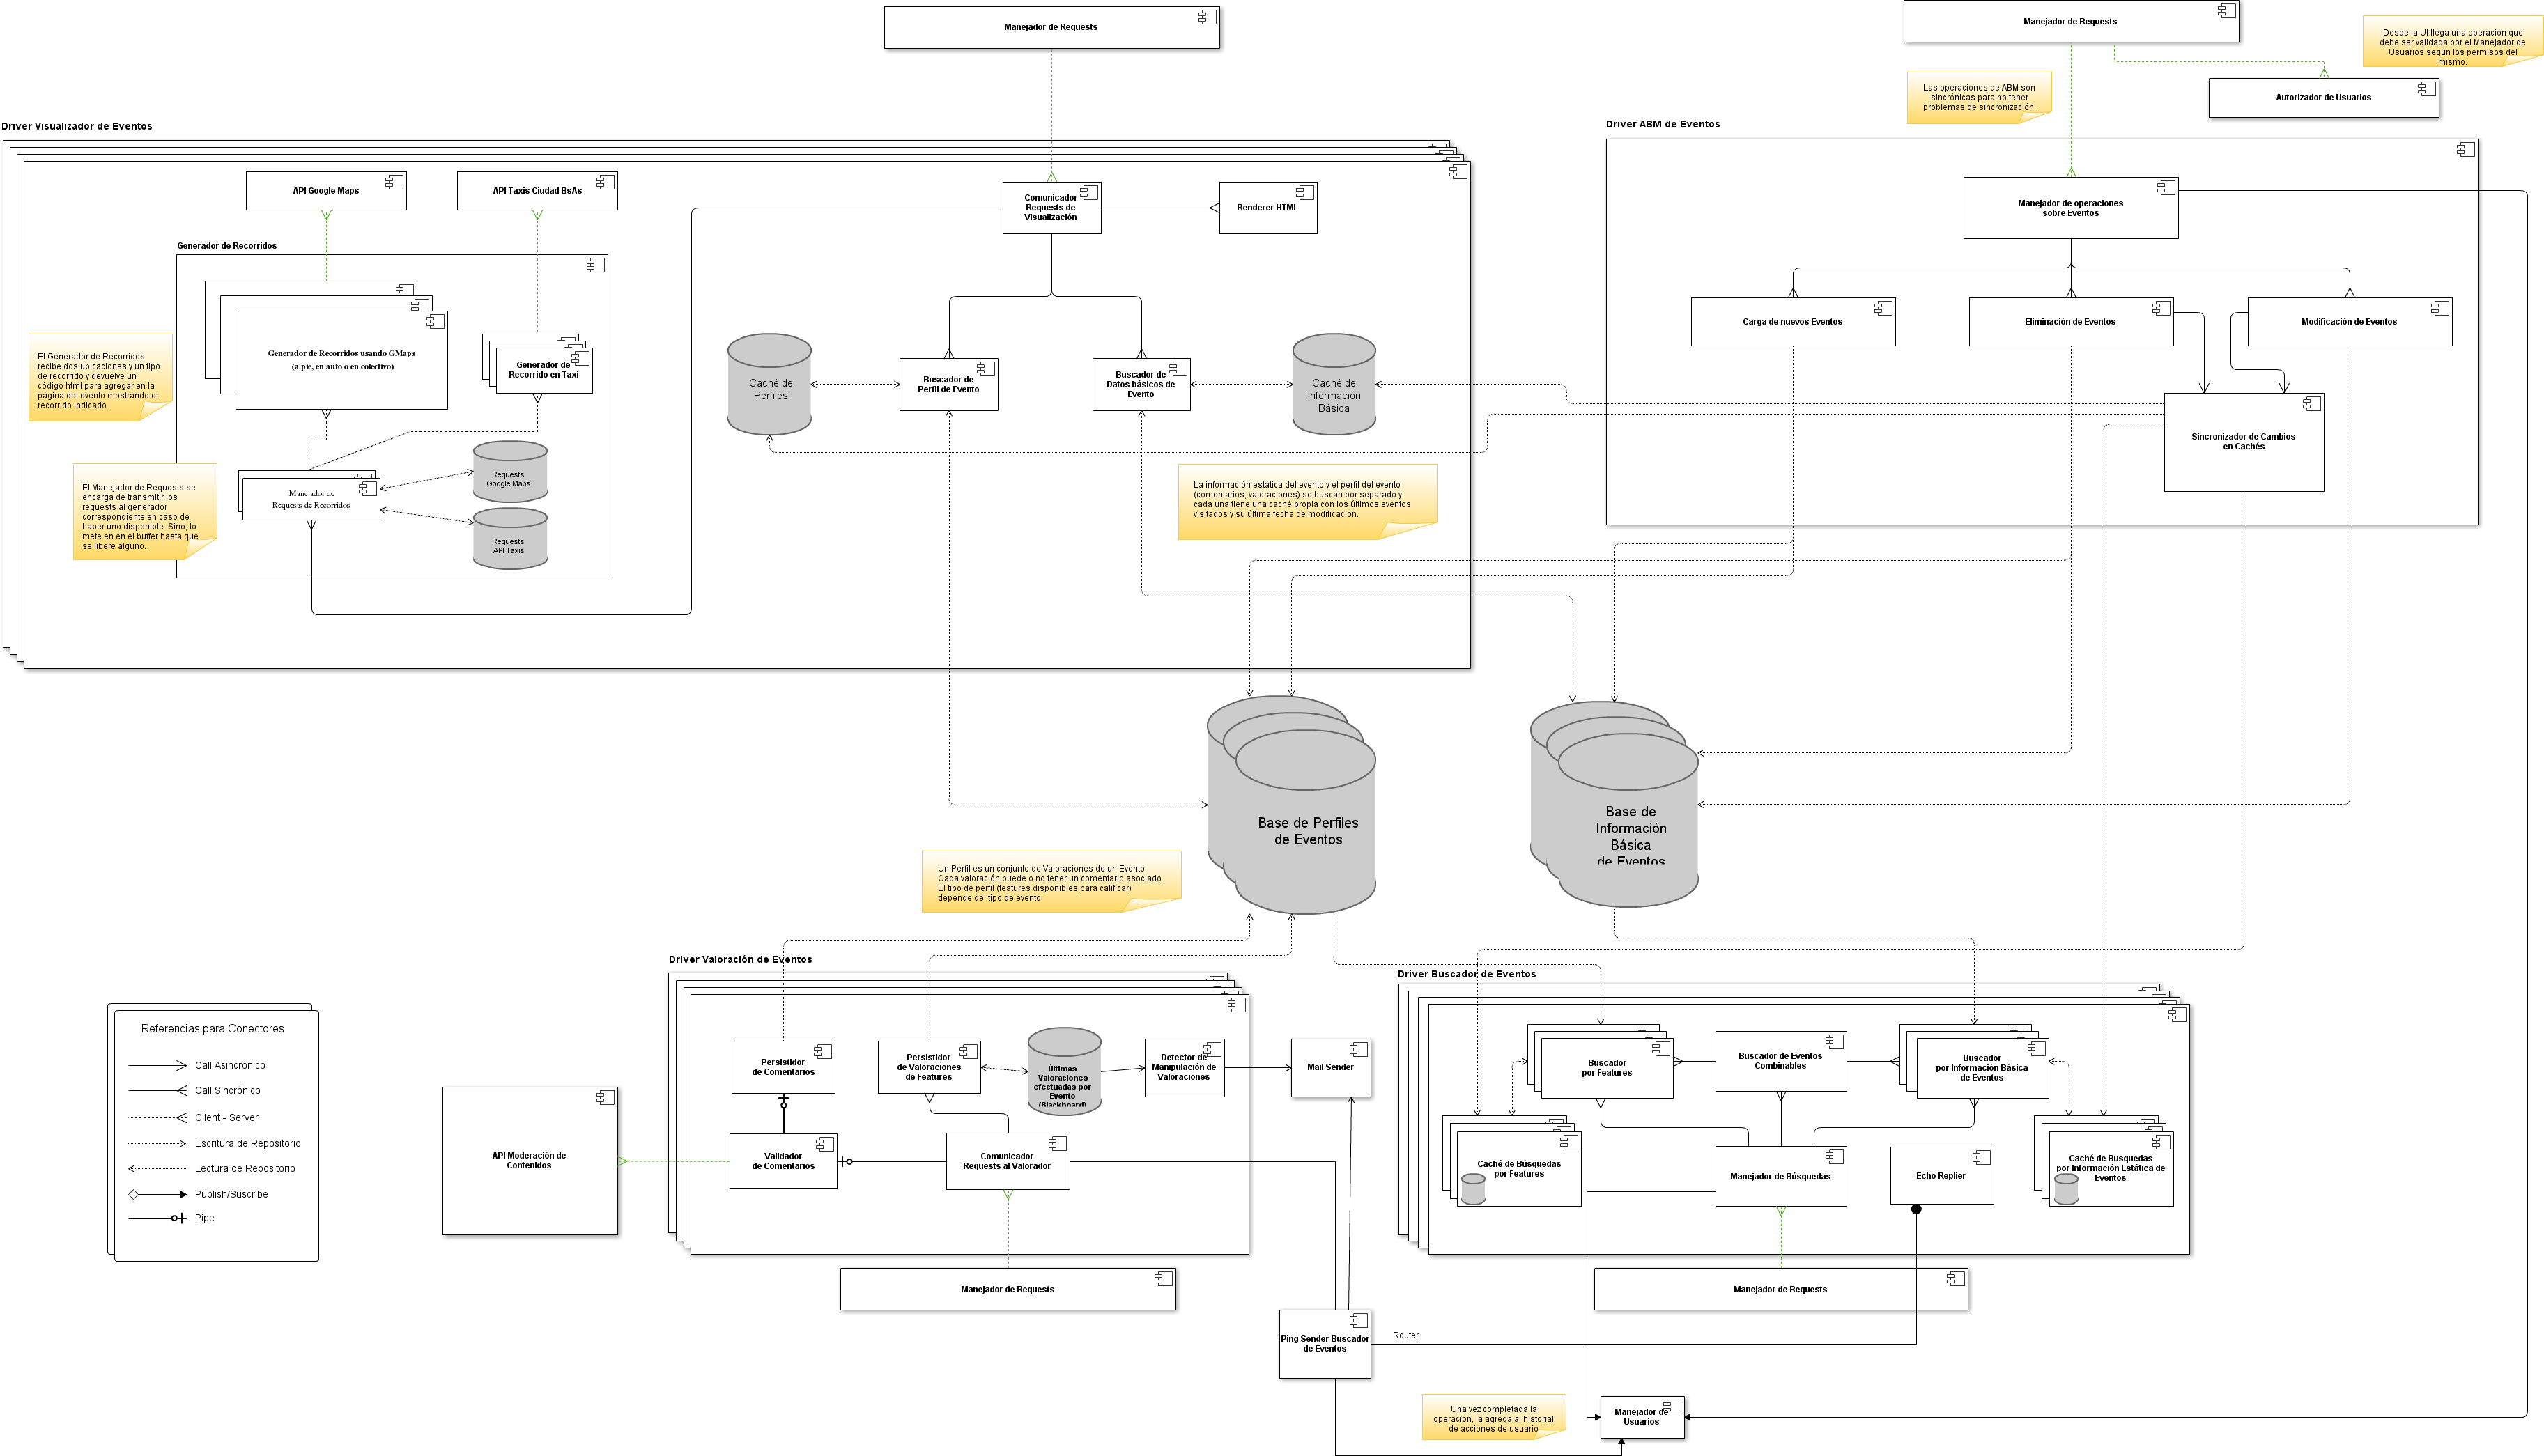
\includegraphics[width=\textwidth]{diagramas/ManejadorDeEventos.png}
  \caption{\normalfont Vista del Manejador de Eventos}
\end{figure} 

\subsubsection{Manejador de Usuarios}

\begin{figure}[H]
  \centering
  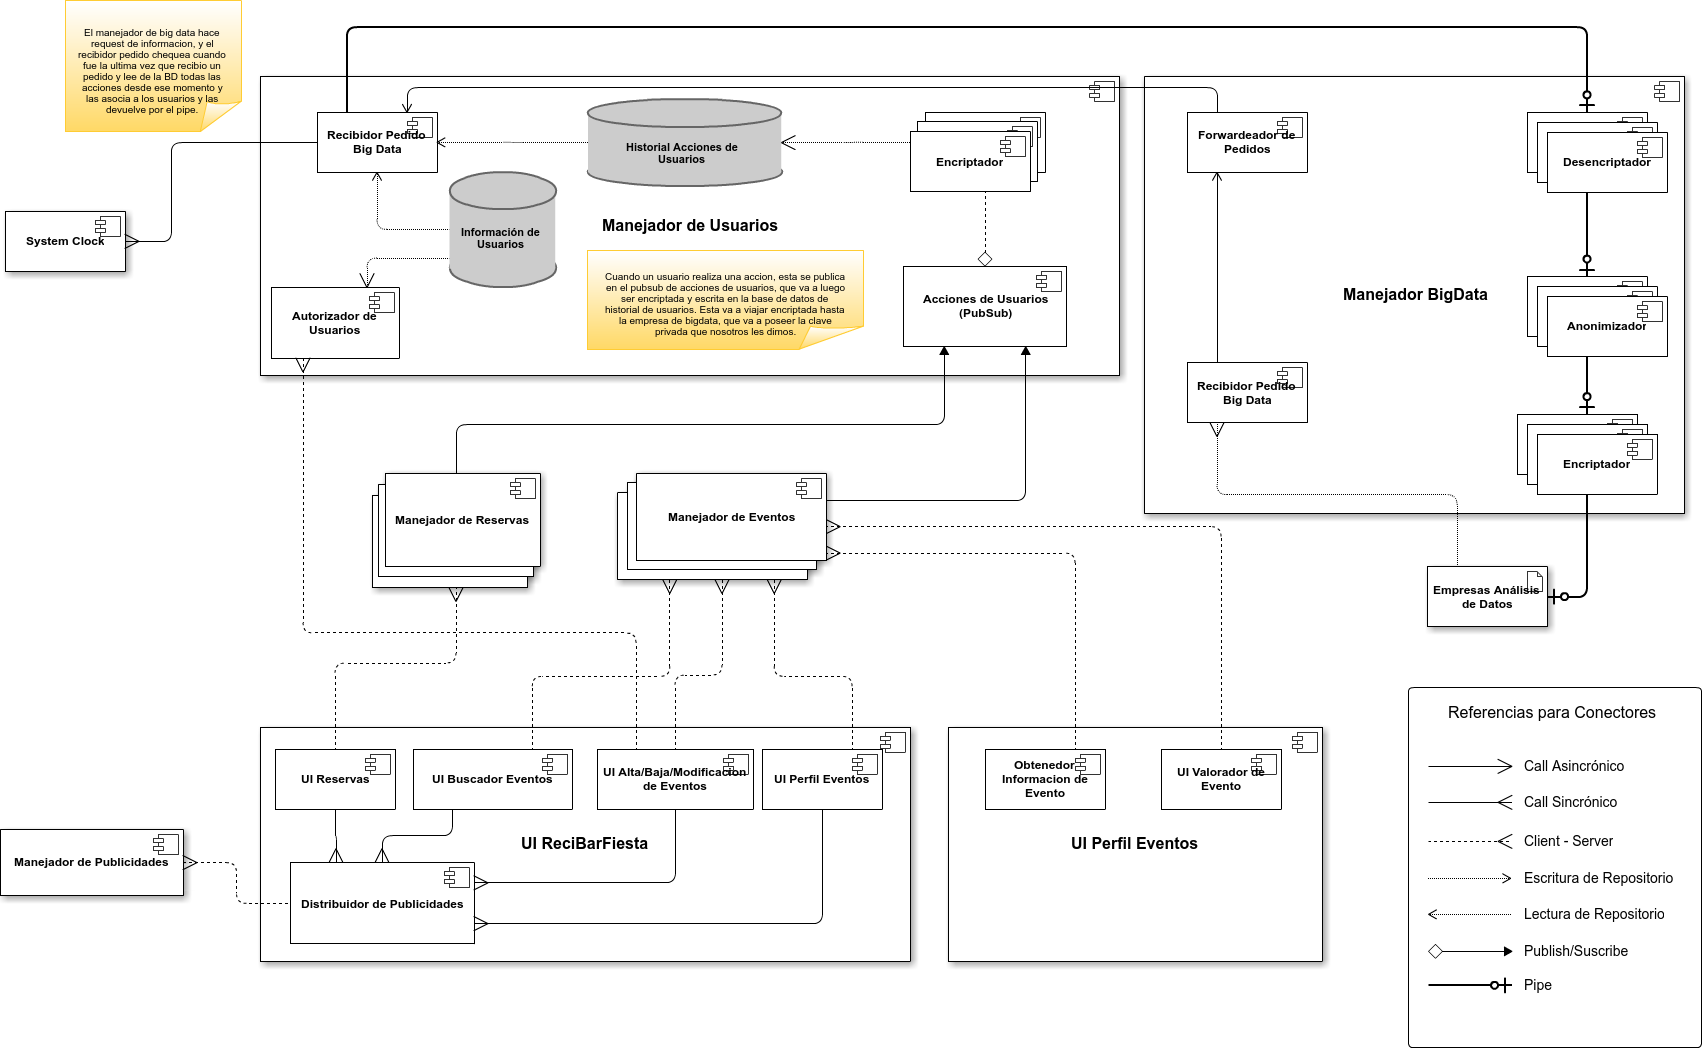
\includegraphics[width=\textwidth]{diagramas/ManejadorDeUsuarios.png}
  \caption{\normalfont Vista del Manejador de Usuarios (con Manejador BigData). Vista de UI ReciBarFiesta. }
\end{figure} 

\subsubsection{Manejador de Reservas}

\begin{figure}[H]
  \centering
  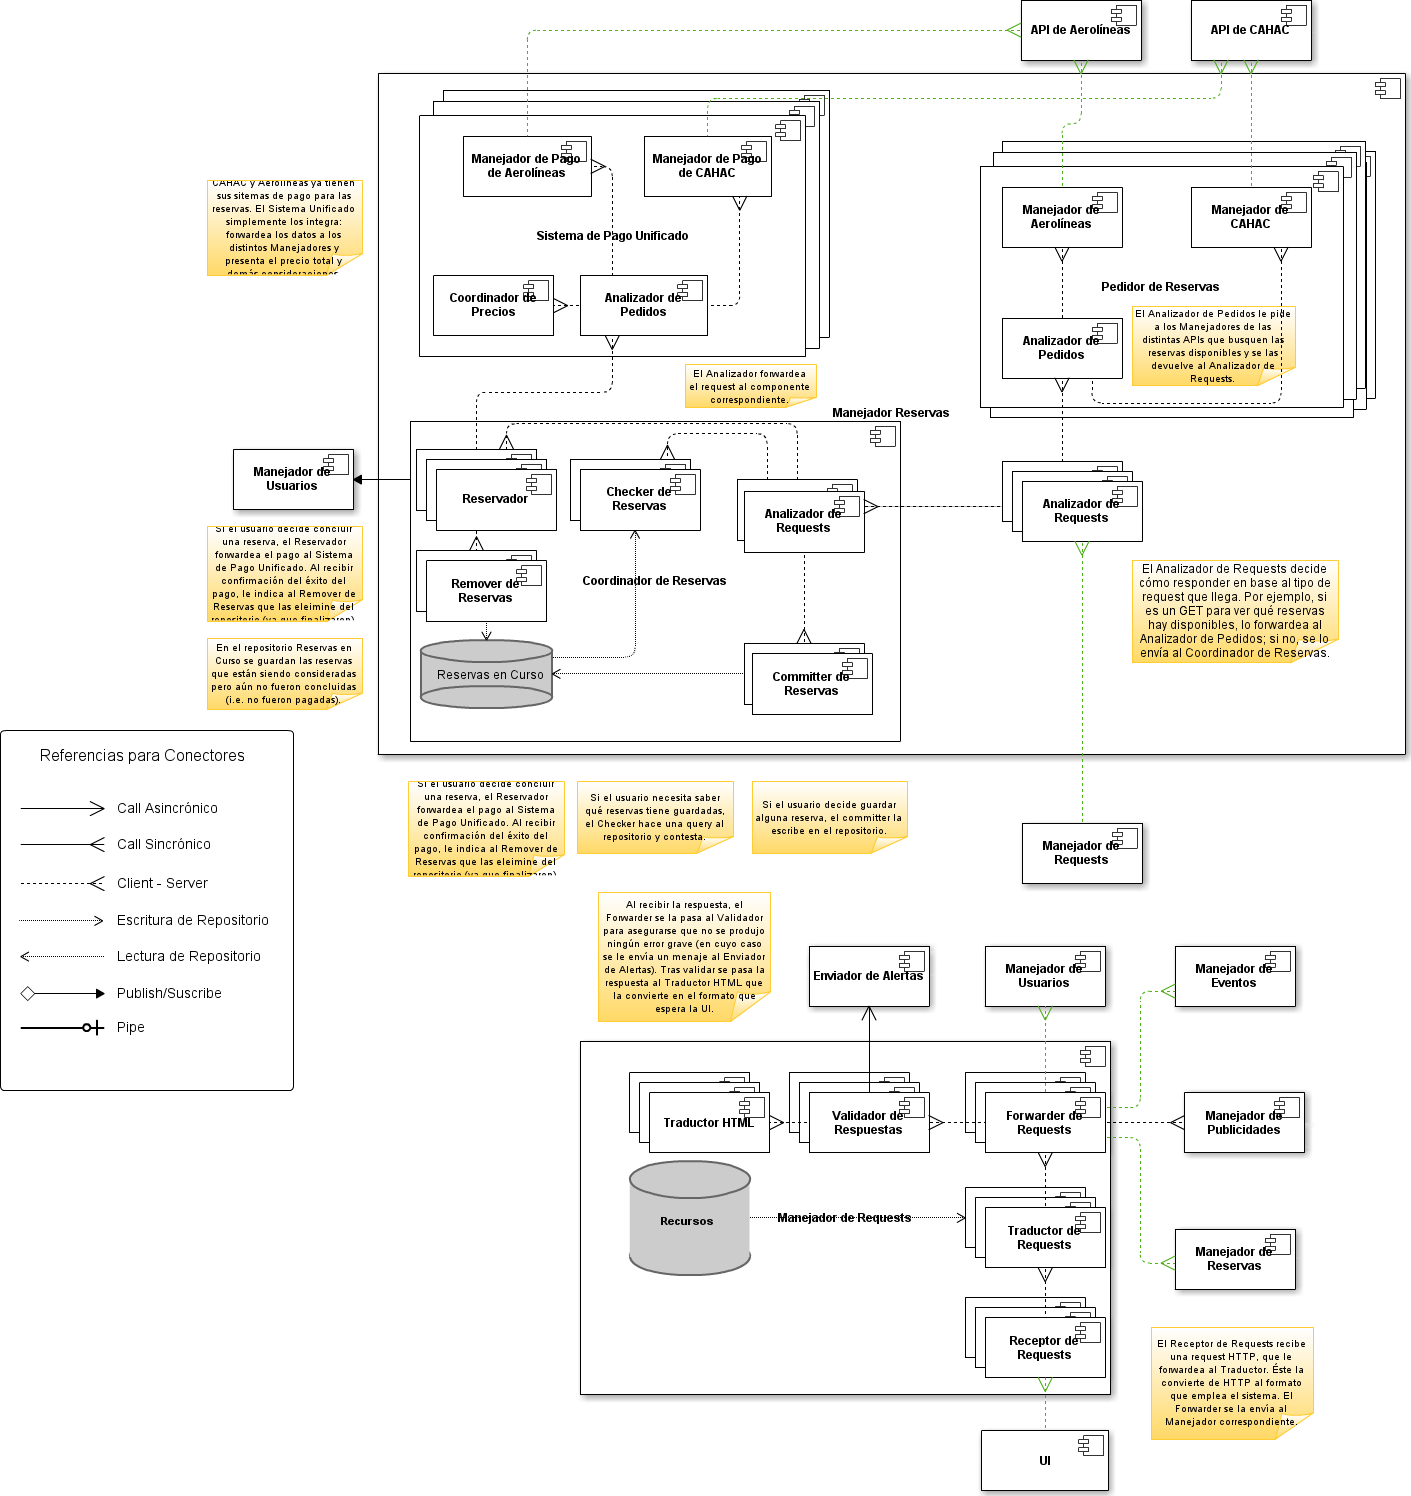
\includegraphics[width=\textwidth]{diagramas/ManejadorReservas.png}
  \caption{\normalfont Vista del Manejador De Reservas.}
\end{figure} 

\subsubsection{Manejador de Publicidades}

\begin{figure}[H]
  \centering
  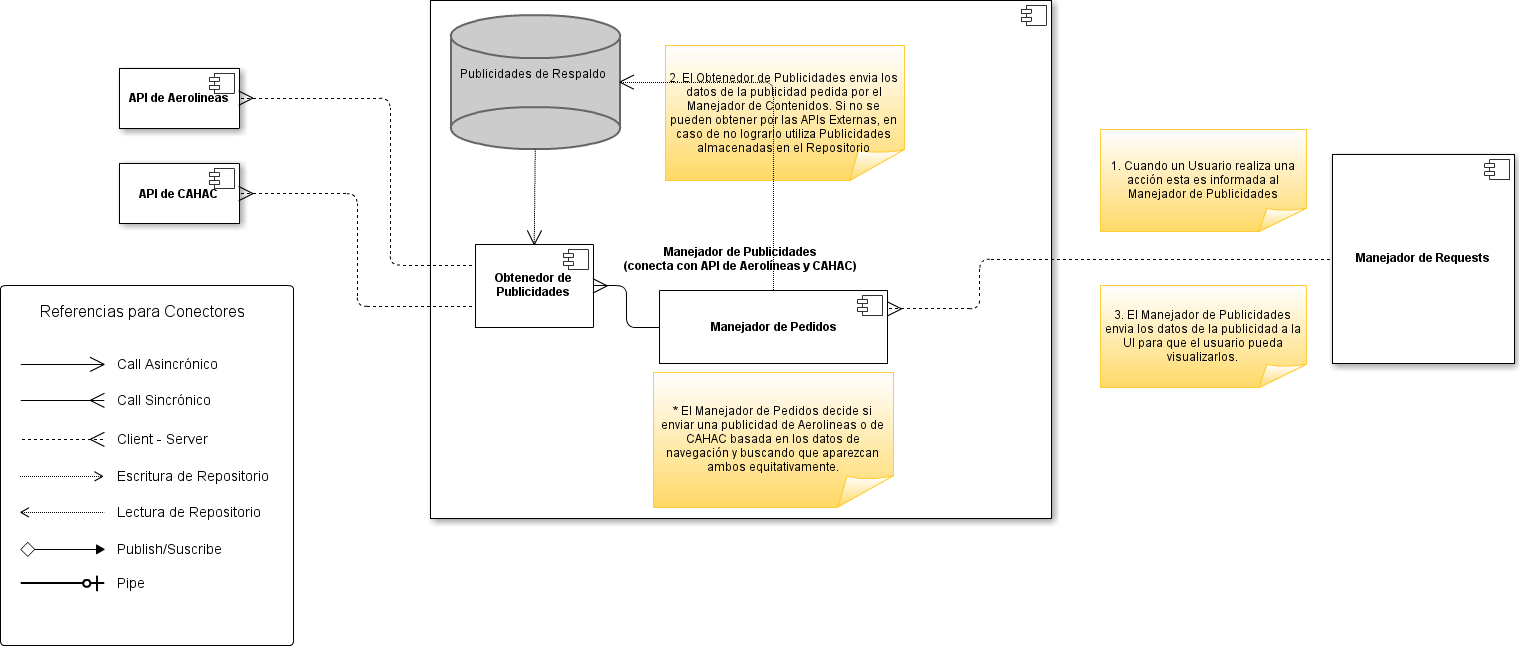
\includegraphics[width=\textwidth]{diagramas/ManejadorDePublicidades.png}
  \caption{\normalfont Vista del Manejador de Publicidades}
\end{figure} 

\subsection{Explicación de la Arquitectura}

\subsubsection{Manejador de Eventos}

El manejador de eventos es el encargado de responder a las distintos requests que envía un usuario de la aplicación desde la interfaz para ejecutar una acción sobre un evento: agregar uno nuevo, modificar, eliminar, valorar, visualizar y búsqueda de eventos.

Notar que los componentes de Visualización, Valoración y Búsqueda de Eventos están replicados para poder realizar muchas operaciones concurrentemente. Sin embargo, el componente de ABM no está replicado para evitar que se generen inconsistencias en la información de los eventos.

\textbf{Visualización de Eventos}

Es el encargado de obtener la información cargada en las bases de datos asociada a un evento en particular, que incluye los datos básicos del evento (así llamaremos a datos como el Nombre, Ubicación, Horario, Tipo de evento, etc.) y los datos del "Perfil del Evento" (que incluye valoraciones por cada feature según el tipo de evento y comentarios asociados a esas valoraciones realizados por los usuarios).

Supongamos que un usuario quiere acceder a la Vista de un evento en particular, al hacer click en un evento el sistema envía el ID del mismo al Manejador, en particular al componente Driver Visualizador de Eventos. Este componente recibe el request y procede a buscar la información asociada al evento (perfil y datos básicos). Para ambos casos, hay un componente encargado de realizar las consultas en la base correspondiente. Además, cada uno tiene una caché asociada con los últimos eventos visitados por los usuarios. Una vez obtenida la información, en caso de que el usuario desee ver el recorrido hasta el evento, se envía al generador de recorridos la dirección actual del usuario y la dirección del evento. Este componente se encargará de interactuar con la API necesaria: GoogleMaps en caso de que sea recorrido a pie, en auto o en colectivo, o la API de Taxis de la Ciudad, para recorridos en taxi. A través de dichas APIs generará un código HTML que se enviará al Comunicador. Luego, el Comunicador del Driver de Visualización envía toda la información al Renderer HTML para generar la página correspondiente y enviársela a la interfaz para que el usuario pueda verla.

\textbf{Alta/Baja/Modificación de Eventos}

Desde la interfaz, un usuario decide realizar una de las operaciones de ABM para algún evento en particular. Primero, el usuario debe ser autorizado por el Autorizador de Usuarios si es que tiene los permisos necesarios para realizar la operación. Una vez chequeados sus permisos, el request llega al Driver ABM de Eventos del Manejador. El Manejador de operaciones deriva el request parseado con los datos necesarios para realizar la operación al componente correspondiente: Carga de nuevos Eventos, Eliminación, o Modificación.
En caso de tratarse de Carga de un Evento, el componente chequea que el evento sea válido, y en caso afirmativo procede a agregarlo a la base de datos de Información básica y a la base de Perfiles, generando un perfil vacío.
En caso de que sea una baja de un evento, el componente elimina todas las entradas del mismo en las bases de perfiles e información básica, y luego envía un request asincrónico al Sincronizador de Cambios en Cachés, encargado de actualizar todas las cachés de los componentes del Manejador de Eventos, para que no queden con datos inconsistentes.
Por último, en caso de ser una modificación, se actualiza la información básica del evento una vez que haya sido validada, y luego se avisa al sincronizador de cachés para que ejecute las actualizaciones.
Una vez finalizada la operación, la misma se guarda en el historial de acciones por usuario.

\textbf{Valorador de Eventos}

Este componente es el encargado de almacenar las valoraciones de los usuarios en el perfil del evento correspondiente. Una valoración debe incluir al menos un valor seleccionable para los features de un evento, que dependen del tipo del mismo, y además puede o no incluir un comentario asociado a dicha valoración. En caso de contener un comentario, éste se encolará para que sea validado interactuando con la API de moderación de contenidos, y luego guardado por el persistidor de Comentarios. En caso de que la conexión con la API se vuelva lenta, se guardará por un lado la valoración y el comentario asociado quedará encolado hasta que sea validado, y luego almacenado. En caso de ocurrir esto se avisará al usuario con mensaje al retornar la respuesta. Si el comentario no es apropiado, se devolverá un mensaje de error. Por otro lado, al persistir las valoraciones, éstas son guardadas temporalmente en un repositorio de últimas valoraciones efectuadas. Este repositorio es leído continuamente por un componente encargado de detectar si se están produciendo demasiadas valoraciones similares al mismo evento; y, en caso de detectarlo, enviará un mail a través del Mail Sender para que la situación sea revisada manualmente.

\textbf{Buscador de Eventos}

El Driver Buscador de Eventos manejará las búsquedas realizadas por los usuarios, dividiéndolas en búsquedas por Features o búsquedas por Información Básica del evento. El Manejador de Búsquedas parseará el request del usuario y enviará la búsqueda al componente Buscador correspondiente según el tipo de la misma. Cada uno de estos componentes cuenta con una Caché donde se almacenarán las búsquedas más populares realizadas por los usuarios, que serán actualizadas periódicamente. Las cachés cuentan con tres niveles (primario, secundario, y terciario) según el nivel de popularidad de las búsquedas para garantizar performance. Una vez realizada la búsqueda, en caso de ser requerido por el usuario, el manejador enviará los resultados al Componente buscador de Eventos Combinables, para que genere búsquedas de eventos combinables (cercanos, temáticas relacionadas, etc.), que luego serán efectuadas por el Buscador correspondiente según se trate de búsquedas en la base de datos de perfiles o de información básica. Una vez obtenidos los resultados, se actualizan las cachés, se notifica al historial de usuario la acción realizada, y se devuelve una página con los resultados y links a las vistas de los eventos encontrados.



\subsubsection{Manejador de Usuarios}

El manejador de usuarios es el componente que se ocupa de todo lo referido a usuarios. Se ocupará, entre otras cosas, de almacenar la información de los usuarios y sus acciones relevantes en la aplicación. 

Interactuará con la empresa de análisis de datos y con la UI de ReciBarFiesta.

\textbf{Acciones de Usuarios (PubSub) y Encriptador}

Estos dos componentes son los más importantes a la hora de guardar las acciones de los usuarios en la aplicación. Cada vez que un usuario haga una accion, el componente que la realiza deberá publicarlo en el PubSub. Hay un encriptador que se ocupa de encriptar los datos y guardarlos en la base de datos de historial de acciones de usuarios. De esta manera la información queda resguardada ante eventuales leaks de información.

\textbf{Manejador BigData}

Este sub-componente de Manejador de Usuarios se ocupa de recibir los pedidos de la empresa de análisis de datos y responderlos. Los pedidos los recibe un Recibidor de Pedidos de Big Data, y es forwardeado por un Forwardeador. Este pedido es recibido por el Recibidor Pedido de Big Data, que chequea cuando fue la última vez que recibió un request y devuelve todas las acciones desde ese momento por un pipe, asociando las acciones con los usuarios, que extrae del repositorio
llamado Información de Usuarios.

Luego, siguiendo un estilo de pipes and filters, esa información es desencriptada, luego anonimizada (se borra la información que permita identificar personas) y luego se encripta nuevamente de manera qu esolo la empresa de análisis de datos pueda leer esos datos. Esto puede hacerse por ejemplo, con un sistema de clave público-privada, muy fácilmente.

\textbf{Autorizador de Usuarios}

Simplemente recibe un usuario y una contraseña y la chequea contra la base de datos de los usuarios, y devuelve un token que podrá utilizar la UI (token de sesión, utilizado por el conector encriptado).


\subsubsection{UI ReciBarFiesta}

\ldots


